%------------------------------------------------------------------------------------
%	PACKAGES AND OTHER DOCUMENT CONFIGURATIONS
%------------------------------------------------------------------------------------

\documentclass{article}

\usepackage{fancyhdr} % Required for custom headers
\usepackage{lastpage} % Required to determine the last page for the footer
\usepackage{extramarks} % Required for headers and footers
\usepackage[usenames,dvipsnames]{color} % Required for custom colors
\usepackage{graphicx} % Required to insert images
\usepackage{subcaption}
\usepackage{listings} % Required for insertion of code
\usepackage{courier} % Required for the courier font
% Optional Packages
\usepackage{amsmath}
\usepackage{amssymb}
\usepackage{float}
\usepackage{algorithm}
\usepackage[noend]{algpseudocode}


% Margins
\topmargin=-0.45in
\evensidemargin=0in
\oddsidemargin=0in
\textwidth=6.5in
\textheight=9.0in
\headsep=0.25in

\linespread{1.1} % Line spacing

% Set up the header and footer
\pagestyle{fancy}
\lhead{\hmwkAuthorName} % Top left header
\chead{\hmwkClass\ : \hmwkTitle} % Top center head
%\rhead{\firstxmark} % Top right header
\lfoot{\lastxmark} % Bottom left footer
\cfoot{} % Bottom center footer
\rfoot{Page\ \thepage\ of\ \protect\pageref{LastPage}} % Bottom right footer
\renewcommand\headrulewidth{0.4pt} % Size of the header rule
\renewcommand\footrulewidth{0.4pt} % Size of the footer rule

\setlength\parindent{0pt} % Removes all indentation from paragraphs


%------------------------------------------------------------------------------------
%	DOCUMENT STRUCTURE COMMANDS
%	Skip this unless you know what you're doing
%------------------------------------------------------------------------------------

% Header and footer for when a page split occurs within a problem environment
\newcommand{\enterProblemHeader}[1]{
	%\nobreak\extramarks{#1}{#1 continued on next page\ldots}\nobreak
	%\nobreak\extramarks{#1 (continued)}{#1 continued on next page\ldots}\nobreak
}

% Header and footer for when a page split occurs between problem environments
\newcommand{\exitProblemHeader}[1]{
	%\nobreak\extramarks{#1 (continued)}{#1 continued on next page\ldots}\nobreak
	%\nobreak\extramarks{#1}{}\nobreak
}

\setcounter{secnumdepth}{0} % Removes default section numbers
\newcounter{homeworkProblemCounter} % Creates a counter to keep track of the number of problems
\setcounter{homeworkProblemCounter}{0}

\newcommand{\homeworkProblemName}{}
\newenvironment{homeworkProblem}[1][Problem \arabic{homeworkProblemCounter}]{ % Makes a new environment called homeworkProblem which takes 1 argument (custom name) but the default is "Problem #"
	\stepcounter{homeworkProblemCounter} % Increase counter for number of problems
	\renewcommand{\homeworkProblemName}{#1} % Assign \homeworkProblemName the name of the problem
	\section{\homeworkProblemName} % Make a section in the document with the custom problem count
	\enterProblemHeader{\homeworkProblemName} % Header and footer within the environment
}{
	\exitProblemHeader{\homeworkProblemName} % Header and footer after the environment
}

\newcommand{\problemAnswer}[1]{ % Defines the problem answer command with the content as the only argument
	\noindent\framebox[\columnwidth][c]{\begin{minipage}{0.98\columnwidth}#1\end{minipage}} % Makes the box around the problem answer and puts the content inside
}

\newcommand{\homeworkSectionName}{}
\newenvironment{homeworkSection}[1]{ % New environment for sections within homework problems, takes 1 argument - the name of the section
	\renewcommand{\homeworkSectionName}{#1} % Assign \homeworkSectionName to the name of the section from the environment argument
	\subsection{\homeworkSectionName} % Make a subsection with the custom name of the subsection
	\enterProblemHeader{\homeworkProblemName\ [\homeworkSectionName]} % Header and footer within the environment
}{
	\enterProblemHeader{\homeworkProblemName} % Header and footer after the environment
}


%=================================================================

%------------------------------------------------------------------------------------
%	NAME AND CLASS SECTION
%------------------------------------------------------------------------------------

\newcommand{\hmwkTitle}{Assignment\ \#4} % Assignment title
\newcommand{\hmwkClass}{CSC321} % Course/class
\newcommand{\hmwkAuthorName}{Xiangyu Kong} % Your name
\newcommand{\hmwkUTorId}{kongxi16} % UTorID

%------------------------------------------------------------------------------------
%	TITLE PAGE
%------------------------------------------------------------------------------------

\title{
	\vspace{2in}
	\textmd{\textbf{\hmwkClass:\ \hmwkTitle}}\\
	%	\normalsize\vspace{0.1in}\small{Due\ on\ \hmwkDueDate}\\
	\vspace{0.1in}
	\vspace{3in}
}

\author{\textbf{\hmwkAuthorName} \\ \textbf{\hmwkUTorId}}

% Insert date here if you want it to appear below your name
\date{\today} 

%------------------------------------------------------------------------------------

\begin{document}
	
	\maketitle
	\clearpage
	
	%---------------------------------------------------------------------------------
	%	PROBLEM 1
	%---------------------------------------------------------------------------------
	\begin{homeworkProblem}
		
		\begin{enumerate}
			\item \large{\textbf{Implement the Discriminator of the DCGAN}}
			\begin{enumerate}
				\item 
				Let $P = \text{number of padding}$, $W = \text{input width}$, $K = \text{kernel size}$, $S = \text{stride}$, $O = \text{output width}$
				
				According to the structure of the convolutional network, 
				\begin{align*}
					O &= \dfrac{W}{2}
				\end{align*}
				
				Using the formula for calculating output dimension
				\begin{align*}
					O &= \frac{W - K + 2P}{S} \\
					P &= \frac{S (\frac{W}{2} - 1) + K - W}{2} \\
						&= \frac{2 (\frac{W}{2} - 1) + 4 - W}{2} \\
						&= \frac{W - 2 + 4 - W}{2} \\
						&= 1
				\end{align*}
				
				\item
				See implementation in models.py
			\end{enumerate}
			
			%-----------------------------------------------------------------------------
			
			\item \large{\textbf{Generator}}\\
			See implementation in models.py
			
			\item \large{\textbf{Experiment}}\\
			Samples from iterations 200 and 5000 are shown in Fig\ref{fig:1}.
			The sample improves in their resolution and quality. We can clearly see what each emoji is (human figure or objects) after a very long period of iterations.
			
			
			\begin{figure*}[!ht]
				\centering
				\begin{subfigure}{.45\textwidth}
					\centering
					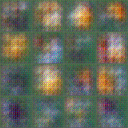
\includegraphics[width=.8\linewidth]{images/sample-000200.png}
					\caption{Sample from iteration 200}
					\label{fig:1.1}
				\end{subfigure}
				\begin{subfigure}{.45\textwidth}
					\centering
					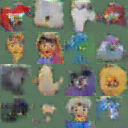
\includegraphics[width=.8\linewidth]{images/sample-005000.png}
					\caption{Sample from iteration 5000}
					\label{fig:1.2}
				\end{subfigure}
				\caption{}
				\label{fig:1}
			\end{figure*}

		\end{enumerate}
		
	\end{homeworkProblem}
	\clearpage
	
	%----------------------------------------------------------------------------------
	
	%---------------------------------------------------------------------------------
	%	PROBLEM 2
	%---------------------------------------------------------------------------------
	\begin{homeworkProblem}

		\begin{enumerate}
			\item \large{\textbf{Generator}}\\
			See implementation in model.py
			
			\item \large{\textbf{CycleGAN Training Loop}}\\
			See implementation in cycle\_gan.py
			
			\item \large{\textbf{CycleGAN Experiments}}
			\begin{enumerate}
				\item 
				The samples without cycle-consistency loss at iteration 400 are shown in Fig\ref{fig:2}
				
				\begin{figure*}[!ht]
					\centering
					\begin{subfigure}{.45\textwidth}
						\centering
						
\includegraphics[width=.8\linewidth]{images/sample-000400-X-Y.png}
						\caption{Sample from iteration 200}
						\label{fig:2.1}
					\end{subfigure}
					\begin{subfigure}{.45\textwidth}
						\centering
						
\includegraphics[width=.8\linewidth]{images/sample-000400-Y-X.png}
						\caption{Sample from iteration 5000}
						\label{fig:2.2}
					\end{subfigure}
					\caption{}
					\label{fig:2}
				\end{figure*}
				
				\item 
				The samples with cycle-consistency loss at iteration 400 are shown in Fig\ref{fig:3}
				
				\begin{figure*}[!ht]
					\centering
					\begin{subfigure}{.45\textwidth}
						\centering
						
\includegraphics[width=.8\linewidth]{images/sample-000400-X-Y.png}
						\caption{Sample from iteration 200}
						\label{fig:3.1}
					\end{subfigure}
					\begin{subfigure}{.45\textwidth}
						\centering
						
\includegraphics[width=.8\linewidth]{images/sample-000400-Y-X.png}
						\caption{Sample from iteration 5000}
						\label{fig:3.2}
					\end{subfigure}
					\caption{}
					\label{fig:3}
				\end{figure*}
				
				\item 
				The samples from the pre-trained network without cycle-consistency loss are shown in Fig\ref{fig:4}
				
				\begin{figure*}[!ht]
					\centering
					\begin{subfigure}{.45\textwidth}
						\centering
						
\includegraphics[width=.8\linewidth]{images/sample-000100-X-Y.png}
						\caption{Sample from iteration 200}
						\label{fig:4.1}
					\end{subfigure}
					\begin{subfigure}{.45\textwidth}
						\centering
						
\includegraphics[width=.8\linewidth]{images/sample-000100-Y-X.png}
						\caption{Sample from iteration 5000}
						\label{fig:4.2}
					\end{subfigure}
					\caption{}
					\label{fig:4}
				\end{figure*}
				
				\item 
				The samples from the pre-trained network with cycle-consistency loss are shown in Fig\ref{fig:4}
				
				\begin{figure*}[!ht]
					\centering
					\begin{subfigure}{.45\textwidth}
						\centering
						
\includegraphics[width=.8\linewidth]{images/sample-000100-X-Y.png}
						\caption{Sample from iteration 200}
						\label{fig:5.1}
					\end{subfigure}
					\begin{subfigure}{.45\textwidth}
						\centering
						
\includegraphics[width=.8\linewidth]{images/sample-000100-Y-X.png}
						\caption{Sample from iteration 5000}
						\label{fig:5.2}
					\end{subfigure}
					\caption{}
					\label{fig:5}
					\end{figure*}
				
				\item 
			\end{enumerate}
		\end{enumerate}
				
	\end{homeworkProblem}
	\clearpage
	
	%----------------------------------------------------------------------------------
	
\end{document}